\documentclass{article}
\usepackage[margin=1in]{geometry}
\usepackage{amsmath}
\usepackage{booktabs}
\usepackage{siunitx}
\usepackage{tikz}
\usetikzlibrary{arrows.meta, positioning, shapes.geometric}
\begin{document}

\title{Design Calculations: Fuzzy Scheduler Workflow}
\author{}
\date{}
\maketitle

\section{Objective / Purpose Statement}
Design objective: maximize line-following speed while keeping lateral error stable and avoiding loss of the line. 
Constraint: motor speed is capped by hardware and the camera can only observe a limited lookahead length. 
Design decision: use a fuzzy scheduler that maps the current speed command and the visible line length into a speed cap and PID gains.

\section{References}
\begin{itemize}
\item ``A Fuzzy Rule-Based Control System for Fast Line-Following Robots,'' DCOSS 2020.
\item MTE 380 Detailed Design W2026 (design calculation template guidance).
\end{itemize}

\section{Design Inputs}
\begin{itemize}
\item $x_{j,k}$: commanded speed of motor $j$ at iteration $k$.
\item $|X|$: maximum motor speed capability (rpm).
\item $L_k$: length of the currently detected line segment from the camera.
\item $|L|$: maximum detectable line length for the camera (within the ROI).
\item $e$: lateral error from IR array (weighted centroid error).
\item Membership function breakpoints for $X_1$, $X_2$, and output labels (heuristic, tunable).
\end{itemize}

\section{Assumptions}
\begin{itemize}
\item The camera reliably segments the line in the bottom ROI under expected lighting.
\item $L_k$ is computed as the number of ROI rows containing line pixels and is proportional to visible line length.
\item The control loop runs fast enough that $e$ and $L_k$ are representative of the current state.
\item Integral gain $K_i$ is set to 0 in the initial tuning to avoid wind-up; this can be revisited.
\end{itemize}

\section{Signal Processing: Computing $X_1$ and $X_2$}
The fuzzy scheduler inputs come from the IR array and the camera:
\begin{itemize}
\item \textbf{IR array (lateral error):} read the IR sensor values, compute the weighted centroid of the line, and subtract the array center to obtain lateral error $e$ used by the PID controller. The IR array does not directly provide $X_1$; it provides the feedback error that the PID corrects.
\item \textbf{Camera (visible line length):} threshold the bottom ROI of the frame to isolate the line, count the number of ROI rows that contain line pixels, and define
\[
L_k = \text{rows with line pixels}, \quad |L| = \text{ROI height}.
\]
Then $X_2 = \frac{L_k}{|L|}\times 100$ (line length percentage).
\item \textbf{Speed command:} $X_1$ is the current forward speed command (or PWM command) normalized to percent of the maximum motor speed,
\[
X_1 = \frac{\max_j x_{j,k}}{|X|}\times 100.
\]
In the absence of encoders, the commanded speed is used as a proxy for actual speed.
\end{itemize}

\section{Analytical Method and Computations}
The fuzzy scheduler follows the DCOSS 2020 method. Two normalized inputs feed six rules; the aggregated output is defuzzified to a scalar $X^*$ (range 1--100). The winning output label maps to a speed cap and PID gains for the downstream controller.

\subsection*{Fuzzy Process Flowchart}
\begin{center}
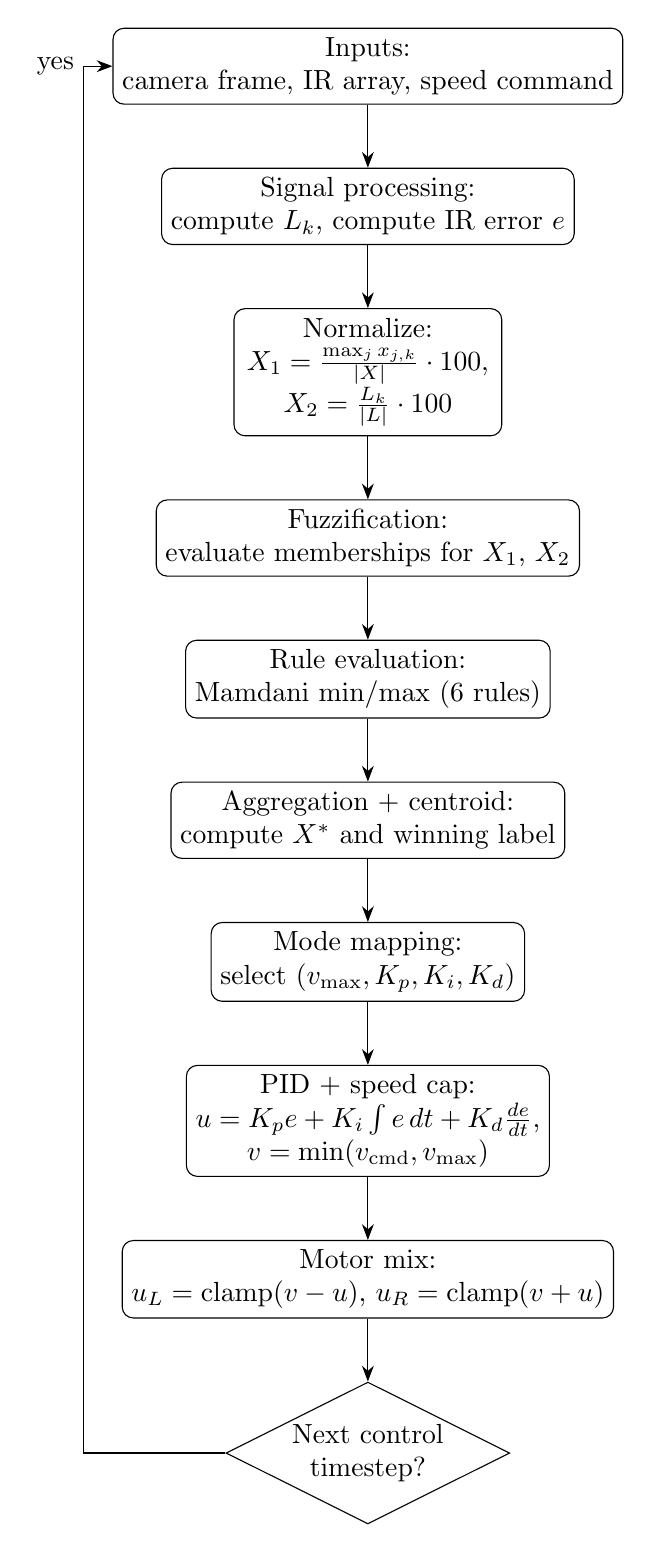
\begin{tikzpicture}[
    node distance=8mm and 14mm,
    block/.style={rectangle, rounded corners, draw, align=center, minimum width=34mm, minimum height=8mm},
    decision/.style={diamond, draw, aspect=2, align=center, inner sep=1pt},
    arrow/.style={-{Stealth[length=2mm]}}
]
    \node[block] (in) {Inputs:\\camera frame, IR array, speed command};
    \node[block, below=of in] (sig) {Signal processing:\\compute $L_k$, compute IR error $e$};
    \node[block, below=of sig] (norm) {Normalize:\\$X_1=\frac{\max_j x_{j,k}}{|X|}\cdot100$,\\$X_2=\frac{L_k}{|L|}\cdot100$};
    \node[block, below=of norm] (fuzz) {Fuzzification:\\evaluate memberships for $X_1$, $X_2$};
    \node[block, below=of fuzz] (rule) {Rule evaluation:\\Mamdani min/max (6 rules)};
    \node[block, below=of rule] (agg) {Aggregation + centroid:\\compute $X^*$ and winning label};
    \node[block, below=of agg] (map) {Mode mapping:\\select $(v_{\max}, K_p, K_i, K_d)$};
    \node[block, below=of map] (pid) {PID + speed cap:\\$u=K_p e + K_i\int e\,dt + K_d\frac{de}{dt}$,\\$v=\min(v_{\text{cmd}}, v_{\max})$};
    \node[block, below=of pid] (mix) {Motor mix:\\$u_L=\text{clamp}(v-u)$, $u_R=\text{clamp}(v+u)$};
    \node[decision, below=of mix] (next) {Next control\\timestep?};

    \draw[arrow] (in) -- (sig);
    \draw[arrow] (sig) -- (norm);
    \draw[arrow] (norm) -- (fuzz);
    \draw[arrow] (fuzz) -- (rule);
    \draw[arrow] (rule) -- (agg);
    \draw[arrow] (agg) -- (map);
    \draw[arrow] (map) -- (pid);
    \draw[arrow] (pid) -- (mix);
    \draw[arrow] (mix) -- (next);
    \draw[arrow] (next.west) -- ++(-18mm,0) |- node[left]{yes} (in.west);
\end{tikzpicture}
\end{center}

\subsection*{Input normalization}
From the paper, the fuzzy inputs are normalized as:
\begin{align}
X_1 &= \frac{\max_j x_{j,k}}{|X|}\times 100, \quad j\in[1,\ldots,N] \\
X_2 &= \frac{L_k}{|L|}\times 100
\end{align}
In this repository:
\begin{itemize}
\item $X_1$: current forward speed command in $[0,1]$ multiplied by 100.
\item $X_2$: fraction of ROI rows containing line pixels (``len\_pct'' in \texttt{vision.py}) as a percentage.
\end{itemize}

\subsection*{Membership functions}
Triangular membership function:
\[
\mu_{\triangle}(x;a,b,c)=
\begin{cases}
0,& x\le a \text{ or } x\ge c\\
\dfrac{x-a}{b-a},& a<x<b\\
\dfrac{c-x}{c-b},& b\le x<c
\end{cases}
\]

\paragraph*{Input $X_1$ (motor speed \%)}
\begin{center}
\begin{tabular}{lll}
\toprule
Label & Triangle $(a,b,c)$ & Notes\\
\midrule
Low    & $(0,0,40)$  & rises to 1 at 0, falls to 0 at 40\\
Medium & $(20,50,80)$& centered at 50\\
High   & $(60,100,100)$& starts at 60, flat to 100\\
\bottomrule
\end{tabular}
\end{center}

\paragraph*{Input $X_2$ (line length \%)}
\begin{center}
\begin{tabular}{lll}
\toprule
Label & Triangle $(a,b,c)$ & Notes\\
\midrule
Close & $(0,0,50)$\\
Far   & $(30,100,100)$\\
\bottomrule
\end{tabular}
\end{center}

\paragraph*{Output sets (speed level)}
Labels: LC, LF, MC, MF, HC, HF with triangles:
\[
\begin{aligned}
\text{LC}&:(0,10,25),\quad
\text{LF}:(15,30,45),\quad
\text{MC}:(35,50,65),\\
\text{MF}&:(55,70,85),\quad
\text{HC}:(70,85,95),\quad
\text{HF}:(85,100,100).
\end{aligned}
\]

\subsection*{Rule base (Table I)}
For each input pair $(X_1, X_2)$:
\begin{center}
\begin{tabular}{lll}
\toprule
$X_1$ & $X_2$ & Output label\\
\midrule
Low    & Close & LC\\
Low    & Far   & LF\\
Medium & Close & MC\\
Medium & Far   & MF\\
High   & Close & HC\\
High   & Far   & HF\\
\bottomrule
\end{tabular}
\end{center}
Rule activation uses fuzzy AND as $\min(\mu_{X_1},\mu_{X_2})$. If multiple rules map to the same output label, fuzzy OR is $\max$ of activations (Mamdani max--min).

\subsection*{Aggregation and defuzzification}
For each sample $x\in[0,100]$ (101 evenly spaced points), compute:
\[
\mu_{\text{agg}}(x)=\max_{L\in \{\text{labels}\}} \min\big(\mu_{\text{rule}}(L),\, \mu_{L}(x)\big).
\]
Centroid defuzzification:
\[
X^* = \frac{\sum_x \mu_{\text{agg}}(x)\, x}{\sum_x \mu_{\text{agg}}(x)}.
\]
Quantize and clamp: $X^*_{\text{q}}=\min(100,\max(1,\text{round}(X^*,2)))$.

\section{Calculations}
\subsection*{Mapping $X^*$ to control parameters}
The winning label (highest activation) selects a speed cap $v_{\max}$ and PID gains $(K_p,K_i,K_d)$ from Table~\ref{tab:pidmap}. The base speed is capped by $v_{\max}$ and the PID correction is applied to generate wheel commands:
\[
u = K_p e + K_i \int e\,dt + K_d \frac{de}{dt}
\]
\[
u_L = \text{clamp}(v - u,\,-1,\,1),\quad
u_R = \text{clamp}(v + u,\,-1,\,1)
\]

\begin{table}[h]
\centering
\begin{tabular}{lcccc}
\toprule
Label & $v_{\max}$ & $K_p$ & $K_i$ & $K_d$\\
\midrule
LC & 0.30 & 0.80 & 0.00 & 0.10\\
LF & 0.35 & 0.70 & 0.00 & 0.10\\
MC & 0.45 & 0.65 & 0.00 & 0.12\\
MF & 0.55 & 0.55 & 0.00 & 0.14\\
HC & 0.65 & 0.45 & 0.00 & 0.16\\
HF & 0.75 & 0.40 & 0.00 & 0.18\\
\bottomrule
\end{tabular}
\caption{PID mapping used in this repo (heuristic), aligned with labels from the paper's Table I.}
\label{tab:pidmap}
\end{table}

\subsection*{Worked example}
Given $X_1=20$ and $X_2=30$:
\begin{enumerate}
\item $\mu_{\text{Low}}(20)=0.5$, $\mu_{\text{Close}}(30)=0.4$; other memberships are 0.
\item Rule Low$\land$Close $\rightarrow$ LC activates with $\min(0.5,0.4)=0.4$.
\item Only LC contributes; its triangle $(0,10,25)$ is clipped at 0.4, centroid over $x\in[0,25]$ yields $X^*=12.04$.
\item Label LC wins; select PID $(0.30, 0.80, 0.00, 0.10)$ and cap the base speed to $v_{\max}=0.30$.
\end{enumerate}

\section{Results / Conclusions}
The calculation converts measurable signals ($X_1$ speed and $X_2$ line length) into a discrete mode that determines a safe speed cap and PID gains. This satisfies the objective of maintaining stable tracking while permitting higher speeds when the visible line is long. The design decision is to use fuzzy scheduling instead of a fixed PID, with tunable membership functions and gain tables that can be refined on hardware.

\section{Underlying Engineering Principle}
The underlying engineering principle is \textbf{feedback control of a dynamic system}. The IR array provides the lateral error for closed-loop PID control, while the camera provides a lookahead measure of line length to adjust controller aggressiveness. The fuzzy system is a rule-based approximation of a nonlinear control law: it maps uncertain, noisy sensor inputs ($X_1$, $X_2$) into stable control parameters (speed cap and gains) using membership functions and defuzzification. This applies control theory concepts of stability, robustness, and sensor fusion rather than relying on a single fixed-gain controller.

\end{document}
